\section{Construction Artifacts in Insertion-Based IPI Data}
\label{sec:artifacts}

We audit a BIPIA-derived dataset, \vtwo{}, built the way insertion-based IPI data is commonly built, and ask how
much of its label can be predicted without reading the inserted content, and whether detectors trained on it use
those cues. All numbers in this section are on the \vtwo{} test split, which is artifact-laden by design of the
audit; fine-tuned results on it are not headline results and appear only next to the shortcut baselines.

\subsection{The \vtwo{} construction}
\vtwo{} uses the EmailQA, TableQA and CodeQA tasks of BIPIA \citep{yi2023bipia}. Documents are deduplicated and split
at the document level, per task, into train, validation and test (70/15/15), so no document appears in two splits.
Train and validation draw attack strings from BIPIA's training attack file and test draws from its disjoint test file;
benign imperative sentences come from two disjoint hand-written pools for train and test. Each document yields four
rows: two injected rows (an attack string inserted), one benign row (a benign imperative inserted), and the raw
document. Classes are balanced exactly per task and split. The test split has \val{VTwoTprTfidfCOneVTwoTestNclusters}
documents, \val{VTwoTprTfidfCOneVTwoTestNclean} clean rows and as many injected rows. The input is
\inp{$q$}{$c$}; for CodeQA, BIPIA provides no question, so every CodeQA row carries the same constant intent.

\paragraph{The artifacts.}
Reading the construction code, rather than the data, gives four label-dependent choices.
\begin{itemize}
  \item \textbf{Position.} Attack strings are inserted either at the start of the document or in the middle;
  benign imperatives are always inserted in the middle; no span is ever inserted at the end. Every row with a span at
  the start is therefore injected.
  \item \textbf{Whitespace.} Middle insertion splits the document on whitespace and re-joins it with single spaces,
  which deletes every newline. Raw documents keep their formatting, start insertions keep it, and every benign row
  loses it, so the presence of a newline is informative about the row type.
  \item \textbf{Span surface form.} Inserted spans differ by class in form: every benign imperative ends in a period
  and none contains a question mark, quotation marks or a newline, whereas attack strings vary on all of these.
  \item \textbf{Template reuse.} A handful of benign templates recur across documents, including a ``Note: \ldots''
  template, and some test-pool benign items are addressed to the model (``Act as a helpful assistant\ldots'',
  ``System: \ldots''), which makes their label ambiguous under any definition.
\end{itemize}
\todo{Row-level leakage: re-establish with committed code (pre-registration P4) before any claim about row-level
splits appears; until then this section claims nothing about leakage.}

\subsection{Content-free baselines}
\label{sec:artifacts:baselines}
Table~\ref{tab:artifact-baselines} reports probes that never see the user request and, except the last, never see
the content of the inserted span. The \emph{position oracle} reads only the recorded insertion mode and predicts
``injected'' for a span at the start. The \emph{first-paragraph rule} is untrained: it flags a row whose first
\verb|\n\n|-separated paragraph has at most 30 words. \emph{Prefix-30} and \emph{suffix-30} are TF-IDF + logistic
regression models on the first or last 30 words of the context. \emph{Span-form} is a logistic regression on nine
content-free features of the inserted span (word and character counts; whether it ends in a question mark,
period or exclamation mark; whether it contains a quote, a digit, or a newline or code character; and its share of
capital letters),
evaluated on the rows that have a span. The learned probes are trained on \vtwo{} train only.

For reference, a TF-IDF + logistic regression detector on the full input reaches macro-F1
\ci{VTwoTfidfCOneFOneMacro} and AUROC \ci{VTwoTfidfCOneRocAuc}. The position field alone reaches macro-F1
\ci{VTwoArtifactPositionOracleFOneMacro}, and the untrained first-paragraph rule
\ci{VTwoArtifactFirstParaRuleFOneMacro}: both CIs lie above chance and below the TF-IDF detector's point estimate.
The first 30 words carry far more signal than the last 30 (\ci{VTwoArtifactPrefixThreeZeroTfidfLrFOneMacro} vs
\ci{VTwoArtifactSuffixThreeZeroTfidfLrFOneMacro}; the CIs do not overlap), which is what the position artifact
predicts. The surface form of the span alone, with no access to its words, gives macro-F1
\ci{VTwoArtifactSpanFormLrFOneMacro} on rows with an inserted span.

\begin{table}[t]
\centering
\resizebox{\columnwidth}{!}{% Generated by scripts/make_tables.py from results/v2_probes/artifact_baselines/20261019-180020_seed42/metrics.json
\begin{tabular}{llrrr}
\toprule
\textbf{Probe} & \textbf{Eval rows} & \textbf{N} & \textbf{Macro-F1 [95\% CI]} & \textbf{ROC-AUC [95\% CI]} \\
\midrule
position\_oracle & v2\_test & 288 & 0.7333 {\scriptsize[0.73, 0.73]} & 0.7500 {\scriptsize[0.75, 0.75]} \\
first\_para\_rule & v2\_test & 288 & 0.7007 {\scriptsize[0.68, 0.72]} & 0.7083 {\scriptsize[0.69, 0.73]} \\
prefix30\_tfidf\_lr & v2\_test & 288 & 0.7046 {\scriptsize[0.68, 0.73]} & 0.7514 {\scriptsize[0.73, 0.78]} \\
suffix30\_tfidf\_lr & v2\_test & 288 & 0.5115 {\scriptsize[0.49, 0.53]} & 0.5236 {\scriptsize[0.51, 0.55]} \\
span\_form\_lr & v2\_test\_inserted\_spans & 216 & 0.8421 {\scriptsize[0.79, 0.89]} & 0.8165 {\scriptsize[0.75, 0.88]} \\
\bottomrule
\end{tabular}
}
\caption{Content-free probes on \vtwo{} test. None reads the user request; the learned probes are trained on
\vtwo{} train. Span-form is evaluated on rows with an inserted span. Brackets: 95\% document-cluster bootstrap CI.}
\label{tab:artifact-baselines}
\end{table}

\subsection{Do trained detectors use position?}
\label{sec:artifacts:probes}
A content-free probe that solves the data shows that a shortcut is available, not that a detector takes it. We
therefore build four stress tests from the \vtwo{} test documents, with a formatting-preserving insertion that splits
only at existing line, sentence or word boundaries and never re-joins words. In each, the same span is placed at the
start, middle and end of the same document, so position effects are paired within document.
\textbf{P1} inserts a neutral declarative sentence (label 0), spliced from another test document of the same task
where possible. \textbf{P2} moves the benign imperative that the document already carries in \vtwo{} (label 0).
\textbf{P3} moves each of the document's two test attacks (label 1). \textbf{P4} applies \vtwo{}'s whitespace
collapse to the raw document and inserts nothing (label 0).

We score a TF-IDF detector, DeBERTa-v3-base \citep{he2021debertav3} fine-tuned on \vtwo{} train (three seeds),
two public content-only detectors (PIGuard \citep{li-etal-2025-piguard} and ProtectAI v2\footnote{Hugging Face
\texttt{protectai/\allowbreak deberta-v3-base-\allowbreak prompt-injection-v2}. \todo{revision used for the \vtwo{} scores}}), and a
Qwen2.5-7B-Instruct LLM judge given the request and the context. The judge's prompt was committed together with
its first scores, so we cannot show that it was fixed before any result was seen; the judges used for our
hypotheses use a separately frozen prompt. Figure~\ref{fig:position} shows the
flag rates and Table~\ref{tab:position-contrasts} the paired contrasts.

\paragraph{Fine-tuned DeBERTa.}
On its own test split, the fine-tuned DeBERTa looks nearly perfect: macro-F1
\val{VTwoTprDebertaMeanVTwoTestFOneMacroMean}~$\pm$~\val{VTwoTprDebertaMeanVTwoTestFOneMacroSd} and AUROC
\val{VTwoTprDebertaMeanVTwoTestRocAucMean}~$\pm$~\val{VTwoTprDebertaMeanVTwoTestRocAucSd} (mean $\pm$ SD over
seeds). The stress tests show that position matters to it. Moving the same benign imperative from the middle to the
start raises its flag rate by \ci{VTwoProbeDebertaMeanPTwoStartMinusMiddle} (seed mean), and the increase is positive
with a CI excluding 0 for every seed. Moving an attack from the start to the end lowers recall (end $-$ start:
\ci{VTwoTruncDebertaMeanPThreeendminusstartFull}).

Part of the end-position drop is truncation: DeBERTa reads \val{VTwoTruncWindowTokens} tokens, and a fraction
\val{VTwoTruncDebertaMeanPThreeendtruncated} of P3 end rows lose part of the span. On the matched subset of
documents whose span is fully visible at all three positions, the end $-$ start difference shrinks to
\ci{VTwoTruncDebertaMeanPThreeendminusstartMatched} but still excludes 0 for every seed, and the P2 contrast is
unchanged (\ci{VTwoTruncDebertaMeanPTwostartminusmiddleMatched}). Training on data in which only attacks appear at
the start produces a detector that treats ``at the start'' as evidence of an attack.

\paragraph{The shortcut depends on the seed.}
The three DeBERTa seeds have overlapping test macro-F1 CIs (Table~\ref{tab:seed-variance}), yet they use position to
different degrees. Even a neutral sentence is flagged more often at the start than in the middle for seed 999
(\ci{VTwoProbeDebertaSNineNineNinePOneStartMinusMiddle}), while for seeds 42 and 123 the difference is
\val{VTwoProbeDebertaSFourTwoPOneStartMinusMiddle} and \val{VTwoProbeDebertaSOneTwoThreePOneStartMinusMiddle}.
The P2 contrast of seed 999 (\ci{VTwoProbeDebertaSNineNineNinePTwoStartMinusMiddle}) does not overlap those of the
other seeds. In-distribution test scores cannot reveal which seed learned the shortcut.

\paragraph{Whitespace.}
P4 isolates the whitespace artifact. The DeBERTa-v3 tokenizer maps a space, \verb|\n| and \verb|\n\n| to the same
tokens and our TF-IDF pipeline collapses whitespace, so neither model can see it: their flag rates on P4 equal those
on the raw documents (P4 $-$ raw clean: \val{VTwoGroupsDebertaMeanPfourminusrawclean} for DeBERTa,
\val{VTwoGroupsTfidfCOnePfourminusrawclean} for TF-IDF). For these models the live artifacts are position and span
form. Whitespace remains visible to any model whose input keeps newlines, such as the LLM judge, for which
P4 $-$ raw clean is \ci{VTwoGroupsJudgeQwenTwoFiveSevenbPfourminusrawclean}.

\paragraph{Detectors not trained on \vtwo{}.}
The public detectors and the judge show a different picture. PIGuard's training data contains most of BIPIA's
training-half attack strings \citep{liu2026passing}, so its \vtwo{} numbers are not zero-shot. Neither public classifier shows a P3
position effect whose CI excludes 0 (PIGuard \ci{VTwoProbePiguardPThreeEndMinusStart}, ProtectAI
\ci{VTwoProbeProtectaiPThreeEndMinusStart}). The LLM judge, which reads the whole input with no truncation, loses
recall towards the end of the document (end $-$ start: \ci{VTwoProbeJudgeQwenTwoFiveSevenbPThreeEndMinusStart}), a position effect
that cannot come from \vtwo{} training. PIGuard catches most \vtwo{} test attacks (recall
\ci{VTwoGroupsPiguardRecall}) and never flags a raw document (\val{VTwoGroupsPiguardRawcleanflag}), but flags
\ci{VTwoGroupsPiguardBenignflag} of the benign imperatives: it separates ``contains an instruction'' from ``contains
none'', which is the strict definition of \S\ref{sec:task}, not the intent-based one. ProtectAI's recall
(\ci{VTwoGroupsProtectaiRecall}) is below its flag rate on raw documents (\ci{VTwoGroupsProtectaiRawcleanflag}).
Table~\ref{tab:test-groups} gives all row groups.

\begin{figure*}[t]
\centering
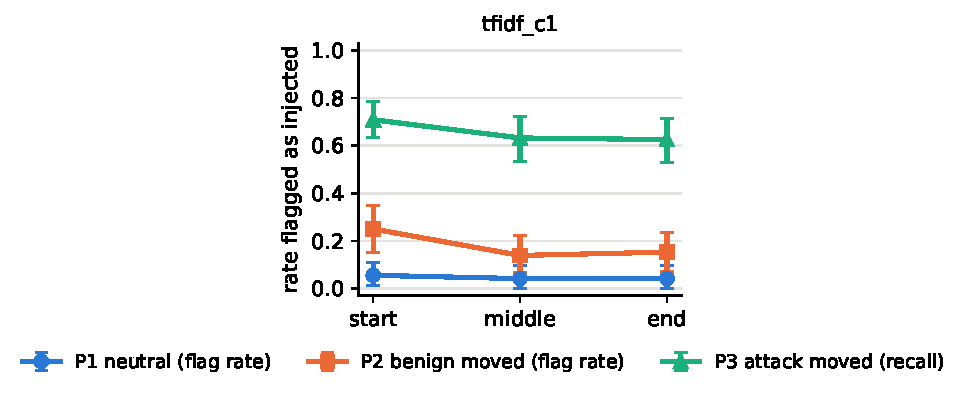
\includegraphics[width=\textwidth]{figures/position_flag_rates.pdf}
\caption{Position stress tests on \vtwo{} test documents. Each panel shows, for one detector, the rate at which
rows are flagged as injected when the same span is placed at the start, middle or end of the same document: a neutral
sentence (P1), the document's benign imperative (P2), and its attacks (P3, recall). Error bars: 95\%
document-cluster bootstrap CI. Default thresholds. \texttt{vsum}: the same judge scored with a rule that sums all
case and whitespace variants of Yes/No.}
\label{fig:position}
\end{figure*}

\begin{table}[t]
\centering
\resizebox{\columnwidth}{!}{% Generated by scripts/make_tables.py from results/v2_probes/probe_report/20261019-180500_seed42/metrics.json
% Paired within-doc differences [paired doc-cluster bootstrap 95% CI]
\begin{tabular}{lrrr}
\toprule
\textbf{Model} & \textbf{P1 start $-$ middle} & \textbf{P3 end $-$ start} & \textbf{P2 start $-$ middle} \\
\midrule
tfidf\_c1 & 0.0139 {\scriptsize[0.00, 0.04]} & -0.0833 {\scriptsize[-0.13, -0.04]} & 0.1111 {\scriptsize[0.06, 0.19]} \\
\bottomrule
\end{tabular}
}
\caption{Paired within-document position contrasts on the stress tests (full probe sets, default threshold).
Brackets: paired document-cluster bootstrap 95\% CI.}
\label{tab:position-contrasts}
\end{table}

\begin{table}[t]
\centering
\resizebox{\columnwidth}{!}{% Generated by scripts/make_tables.py from results/v2_probes/probe_report/20261021-125648_seed42/metrics.json
\begin{tabular}{lrrr}
\toprule
\textbf{DeBERTa seed} & \textbf{V2 test macro-F1} & \textbf{P1 start flag rate} & \textbf{P2 start $-$ middle} \\
\midrule
deberta\_s42 & 0.9514 {\scriptsize[0.93, 0.98]} & 0.0278 {\scriptsize[0.00, 0.07]} & 0.1806 {\scriptsize[0.10, 0.26]} \\
deberta\_s123 & 0.9583 {\scriptsize[0.94, 0.98]} & 0.0417 {\scriptsize[0.00, 0.10]} & 0.1667 {\scriptsize[0.08, 0.25]} \\
deberta\_s999 & 0.9375 {\scriptsize[0.91, 0.97]} & 0.2500 {\scriptsize[0.14, 0.36]} & 0.4167 {\scriptsize[0.31, 0.53]} \\
deberta\_mean & 0.9491 {\scriptsize[0.93, 0.97]} & 0.1065 {\scriptsize[0.06, 0.17]} & 0.2546 {\scriptsize[0.19, 0.32]} \\
\bottomrule
\end{tabular}
}
\caption{Three DeBERTa seeds with indistinguishable \vtwo{} test scores use the position shortcut to different
degrees.}
\label{tab:seed-variance}
\end{table}

\begin{table*}[t]
\centering
\resizebox{\textwidth}{!}{% Generated by scripts/make_tables.py from results/v2_probes/probe_report/20261021-125648_seed42/metrics.json
% V2 test (288 rows, 72 docs) by row group [doc-cluster bootstrap 95% CI]; P4 - raw clean is paired by doc
\begin{tabular}{lrrrrr}
\toprule
\textbf{Model} & \textbf{Recall (injected)} & \textbf{Flag: benign imperative} & \textbf{Flag: raw clean} & \textbf{Flag: P4} & \textbf{P4 $-$ raw clean} \\
\midrule
tfidf\_c1 & 0.6597 {\scriptsize[0.57, 0.74]} & 0.1528 {\scriptsize[0.07, 0.25]} & 0.0694 {\scriptsize[0.01, 0.14]} & 0.0694 {\scriptsize[0.01, 0.12]} & 0.0000 {\scriptsize[0.00, 0.00]} \\
deberta\_s42 & 0.9306 {\scriptsize[0.89, 0.97]} & 0.0556 {\scriptsize[0.01, 0.11]} & 0.0000 {\scriptsize[0.00, 0.00]} & 0.0000 {\scriptsize[0.00, 0.00]} & 0.0000 {\scriptsize[0.00, 0.00]} \\
deberta\_s123 & 0.9514 {\scriptsize[0.92, 0.99]} & 0.0694 {\scriptsize[0.01, 0.14]} & 0.0000 {\scriptsize[0.00, 0.00]} & 0.0000 {\scriptsize[0.00, 0.00]} & 0.0000 {\scriptsize[0.00, 0.00]} \\
deberta\_s999 & 0.9653 {\scriptsize[0.94, 0.99]} & 0.1806 {\scriptsize[0.10, 0.28]} & 0.0000 {\scriptsize[0.00, 0.00]} & 0.0000 {\scriptsize[0.00, 0.00]} & 0.0000 {\scriptsize[0.00, 0.00]} \\
deberta\_mean & 0.9491 {\scriptsize[0.92, 0.98]} & 0.1019 {\scriptsize[0.05, 0.17]} & 0.0000 {\scriptsize[0.00, 0.00]} & 0.0000 {\scriptsize[0.00, 0.00]} & 0.0000 {\scriptsize[0.00, 0.00]} \\
protectai & 0.0903 {\scriptsize[0.03, 0.15]} & 0.1944 {\scriptsize[0.11, 0.29]} & 0.1806 {\scriptsize[0.10, 0.28]} & 0.1667 {\scriptsize[0.08, 0.25]} & -0.0139 {\scriptsize[-0.04, 0.00]} \\
piguard & 0.9236 {\scriptsize[0.88, 0.97]} & 0.7500 {\scriptsize[0.64, 0.86]} & 0.0000 {\scriptsize[0.00, 0.00]} & 0.0000 {\scriptsize[0.00, 0.00]} & 0.0000 {\scriptsize[0.00, 0.00]} \\
judge\_qwen2.5\_7b & 0.3403 {\scriptsize[0.26, 0.42]} & 0.3889 {\scriptsize[0.28, 0.51]} & 0.2083 {\scriptsize[0.11, 0.29]} & 0.2222 {\scriptsize[0.12, 0.32]} & 0.0139 {\scriptsize[-0.06, 0.08]} \\
\bottomrule
\end{tabular}
}
\caption{\vtwo{} test by row group: recall on injected rows, flag rates on benign-imperative rows, raw documents
and their whitespace-collapsed version (P4), and the paired P4 $-$ raw clean difference. Default thresholds.}
\label{tab:test-groups}
\end{table*}

\subsection{Summary}
In \vtwo{}, where a span is inserted and what it looks like predict the label without its content, and a
fine-tuned detector with near-perfect test scores uses insertion position to a degree that varies across seeds and
is invisible in those scores. These are properties of the construction procedure, so any detector trained or
compared on data built this way is affected. \S\ref{sec:v3} removes them.
